\documentclass[aspectratio=169, 12pt]{beamer}
\usepackage[UTF8]{ctex}
\usepackage{graphicx}
\usepackage{booktabs}
\usepackage{listings}
\usepackage{xcolor}
\usepackage{tikz}
\usepackage{hyperref}

% 主题设置
\usetheme{Madrid}
\usecolortheme{whale}
\usefonttheme{professionalfonts}

% 代码高亮设置
\lstset{
    language=Python,
    basicstyle=\ttfamily\small,
    keywordstyle=\color{blue},
    commentstyle=\color{green!60!black},
    stringstyle=\color{orange},
    breaklines=true,
    frame=single,
    showstringspaces=false,
    backgroundcolor=\color{gray!10}
}

% 标题信息
\title[计算机视觉导论与图像基础]{第1周:计算机视觉导论与图像基础}
\subtitle{机器是怎么"看见"试卷的?}
\author{计算机视觉课程组}
\institute{通选课}
\date{}

\begin{document}

% -----------------------------------------------------------------------------
% 标题页
% -----------------------------------------------------------------------------
\begin{frame}
    \titlepage
\end{frame}

% -----------------------------------------------------------------------------
% 目录页
% -----------------------------------------------------------------------------
\begin{frame}{课程概览}
    \tableofcontents
\end{frame}

% -----------------------------------------------------------------------------
% 第一部分:课程导论
% -----------------------------------------------------------------------------
\section{计算机视觉导论}

\begin{frame}{什么是计算机视觉?}
    \begin{block}{定义}
        计算机视觉是一门研究如何使机器"看"的科学,指用摄影机和电脑代替人眼对目标进行识别、跟踪和测量等机器视觉,并进一步做图形处理。
    \end{block}

    \vspace{0.5cm}

    \begin{columns}
        \column{0.5\textwidth}
        \textbf{核心问题:}
        \begin{itemize}
            \item 机器如何"看见"世界?
            \item 图像 $\to$ 数字 $\to$ 理解
        \end{itemize}

        \column{0.5\textwidth}
        \begin{center}
            \begin{tikzpicture}
                \node[draw, circle, fill=blue!20] (img) at (0,2) {图像};
                \node[draw, circle, fill=green!20] (num) at (2,2) {数字};
                \node[draw, circle, fill=red!20] (und) at (4,2) {理解};
                \draw[->, thick] (img) -- (num);
                \draw[->, thick] (num) -- (und);
            \end{tikzpicture}
        \end{center}
    \end{columns}
\end{frame}

\begin{frame}{CV应用领域}
    \begin{columns}
        \column{0.5\textwidth}
        \begin{itemize}
            \item \textbf{安防监控}
                \begin{itemize}
                    \item 人脸识别
                    \item 行为分析
                \end{itemize}
            \item \textbf{自动驾驶}
                \begin{itemize}
                    \item 车道检测
                    \item 障碍物识别
                \end{itemize}
            \item \textbf{医疗影像}
                \begin{itemize}
                    \item 肿瘤检测
                    \item 病灶定位
                \end{itemize}
        \end{itemize}

        \column{0.5\textwidth}
        \begin{itemize}
            \item \textbf{工业检测}
                \begin{itemize}
                    \item 缺陷检测
                    \item 质量分拣
                \end{itemize}
            \item \textbf{教育领域}
                \begin{itemize}
                    \item \textbf{自动阅卷系统}
                    \item 作业批改
                \end{itemize}
        \end{itemize}
    \end{columns}
\end{frame}

\begin{frame}{课程目标:造一个AI阅卷助教}
    \begin{center}
        \begin{tikzpicture}[node distance=1.5cm]
            \node[draw, rectangle, rounded corners, fill=blue!10, minimum width=2cm] (eye) {装上眼睛};
            \node[draw, rectangle, rounded corners, fill=yellow!10, minimum width=2cm, right of=eye] (learn) {学会识别};
            \node[draw, rectangle, rounded corners, fill=green!10, minimum width=2cm, right of=learn] (help) {成为助教};

            \draw[->, thick] (eye) -- (learn);
            \draw[->, thick] (learn) -- (help);

            \node[below of=eye, node distance=1cm, font=\footnotesize] {图像基础};
            \node[below of=learn, node distance=1cm, font=\footnotesize] {三种题型};
            \node[below of=help, node distance=1cm, font=\footnotesize] {完整系统};
        \end{tikzpicture}
    \end{center}

    \vspace{0.5cm}

    \textbf{11周路线:}
    \begin{enumerate}
        \item 第1-2周:基础工具(OpenCV + AI编程)
        \item 第3-8周:核心技能(三种题型识别)
        \item 第9-11周:项目实战(完整系统)
    \end{enumerate}
\end{frame}

% -----------------------------------------------------------------------------
% 第二部分:图像的数字表示
% -----------------------------------------------------------------------------
\section{图像的数字表示}

\begin{frame}{图像的数字表示}
    \begin{block}{从物理图像到数字图像}
        \begin{itemize}
            \item 物理图像:连续的光信号分布
            \item 数字图像:离散的像素点阵
        \end{itemize}
    \end{block}

    \vspace{0.3cm}

    \textbf{像素(Pixel):图像的最小单位}

    \vspace{0.3cm}

    \begin{table}
        \centering
        \begin{tabular}{ccc}
            \toprule
            R (红) & G (绿) & B (蓝) \\
            \midrule
            255 & 0 & 0 $\to$ 红色 \\
            0 & 255 & 0 $\to$ 绿色 \\
            0 & 0 & 255 $\to$ 蓝色 \\
            255 & 255 & 255 $\to$ 白色 \\
            0 & 0 & 0 $\to$ 黑色 \\
            \bottomrule
        \end{tabular}
    \end{table}
\end{frame}

\begin{frame}{RGB色彩空间}
    \begin{columns}
        \column{0.6\textwidth}
        \textbf{RGB三通道:}
        \begin{itemize}
            \item R(Red):红色通道
            \item G(Green):绿色通道
            \item B(Blue):蓝色通道
        \end{itemize}

        \vspace{0.3cm}

        \textbf{数值范围:} 0-255(8位无符号整数)
        \begin{itemize}
            \item 0 = 最暗
            \item 255 = 最亮
        \end{itemize}

        \column{0.4\textwidth}
        \begin{center}
            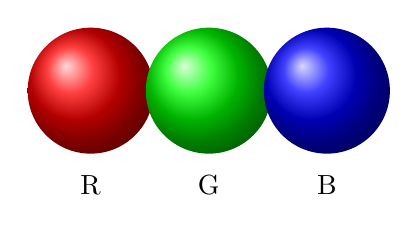
\begin{tikzpicture}
                \shade[ball color=red] (0,0) circle (0.8cm);
                \node at (0,-1.2) {R};
                \shade[ball color=green] (1.5,0) circle (0.8cm);
                \node at (1.5,-1.2) {G};
                \shade[ball color=blue] (3,0) circle (0.8cm);
                \node at (3,-1.2) {B};
            \end{tikzpicture}

            \vspace{0.5cm}

            \textbf{混合 = 各种颜色}
        \end{center}
    \end{columns}
\end{frame}

\begin{frame}[fragile]{OpenCV基础:读取与显示图像}
    \begin{lstlisting}[title={OpenCV基础操作}]
import cv2
import numpy as np

# 读取图像
img = cv2.imread('test.jpg')

# 查看图像信息
print(f"尺寸: {img.shape}")  # (height, width, channels)
print(f"数据类型: {img.dtype}")  # uint8

# 读取灰度图
img_gray = cv2.imread('test.jpg', cv2.IMREAD_GRAYSCALE)

# 显示图像
cv2.imshow('Image', img)
cv2.waitKey(0)
cv2.destroyAllWindows()

# 保存图像
cv2.imwrite('output.jpg', img)
    \end{lstlisting}
\end{frame}

% -----------------------------------------------------------------------------
% 第三部分:动手实验
% -----------------------------------------------------------------------------
\section{动手实验:图像滤镜}

\begin{frame}{实验任务:给试卷加滤镜}
    \textbf{任务目标:}
    \begin{enumerate}
        \item 读取一张试卷图片
        \item 实现3种滤镜效果
        \item 保存并展示结果
    \end{enumerate}

    \vspace{0.3cm}

    \textbf{推荐滤镜:}
    \begin{itemize}
        \item 灰度化
        \item 反色效果
        \item 亮度调整
    \end{itemize}
\end{frame}

\begin{frame}[fragile]{滤镜实现示例}
    \begin{lstlisting}[title={三种滤镜实现}]
import cv2
import numpy as np

img = cv2.imread('exam_paper.jpg')

# 滤镜1:灰度化
gray = cv2.cvtColor(img, cv2.COLOR_BGR2GRAY)

# 滤镜2:反色
inverted = 255 - img

# 滤镜3:调整亮度
bright = np.clip(img.astype(int) + 50, 0, 255).astype(np.uint8)

# 保存结果
cv2.imwrite('gray.jpg', gray)
cv2.imwrite('inverted.jpg', inverted)
cv2.imwrite('bright.jpg', bright)
    \end{lstlisting}
\end{frame}

% -----------------------------------------------------------------------------
% 第四部分:思考题
% -----------------------------------------------------------------------------
\section{思考题}

\begin{frame}{课堂思考题}
    \begin{block}{问题1:图像的数字化}
        \begin{itemize}
            \item 为什么计算机使用RGB三原色?
            \item 为什么像素值范围是0-255?
            \item 如果用更多位(如16位)表示像素,有什么好处?
        \end{itemize}
    \end{block}

    \vspace{0.3cm}

    \begin{block}{问题2:OpenCV基础}
        \begin{itemize}
            \item OpenCV读取的图像为什么是BGR格式?
            \item 如何访问图像中心点的像素值?
        \end{itemize}
    \end{block}
\end{frame}

% -----------------------------------------------------------------------------
% 第五部分:课后作业
% -----------------------------------------------------------------------------
\section{课后作业}

\begin{frame}{课后作业}
    \begin{block}{题目}
        用OpenCV实现3种图像滤镜效果
    \end{block}

    \textbf{项目关联:} 图像滤镜是自动阅卷系统中预处理的基础。例如:灰度化可以简化后续处理,反色可以增强某些特征,对比度调整可以提高识别准确率。

    \textbf{要求:}
    \begin{enumerate}
        \item 必须包含:灰度化、反色
        \item 自选一种:亮度调整、对比度调整、模糊等
        \item 提交:代码 + 处理前后对比图
    \end{enumerate}

    \vspace{0.3cm}

    \textbf{评分标准:}
    \begin{itemize}
        \item 代码正确性:30分
        \item 滤镜实现:40分
        \item 代码规范:15分
        \item 结果展示:15分
    \end{itemize}
\end{frame}

\begin{frame}{下节预告}
    \begin{center}
        \Large \textbf{第2周:AI辅助编程工具实战}

        \vspace{0.5cm}

        \normalsize
        故事问题:\textcolor{blue}{怎么让AI帮我写代码?}

        \vspace{0.3cm}

        你将学会:
        \begin{itemize}
            \item 使用ChatGPT/Claude等AI工具
            \item 编写有效的Prompt
            \item AI辅助代码调试
        \end{itemize}
    \end{center}
\end{frame}

\begin{frame}
    \begin{center}
        \Huge \textbf{谢谢!}

        \vspace{1cm}

        \Large 有问题随时交流
    \end{center}
\end{frame}

\end{document}
